\chapter{Theoretical Background}

This chapter introduces the core concepts underlying this thesis, including building footprint extraction, deep learning architectures, multimodal large language models, and current approaches to quality assessment in GIScience.


\section{Geospatial Data Quality}
\label{sec:geospatial_data_quality}

Geospatial data quality describes the degree to which spatial data are suitable for a given purpose.
\cite{veregin1999data} states that quality usually refers to a high degree of craftsmanship; however, this concept becomes more difficult to apply to data, which lack physical characteristics. Instead, geospatial data quality is commonly described through abstract properties such as accuracy, completeness, consistency, and resolution \citep{veregin1999data}.
These concepts are formalized in the international standard \textit{Geographic information — Data quality} (ISO~19157-1:2023), which defines a structured framework for describing and documenting geospatial data quality \citep{ISO19157-1:2023}. The standard specifies five core quality elements: completeness, logical consistency, positional accuracy, temporal quality, and thematic quality. Related work often uses slightly different terminology. For example, \citep{Vieira_dataqualityindicators} and \cite{dataqualityinEarthobservation} refer to completeness, logical consistency, positional accuracy, temporal accuracy, and attribute accuracy, while also emphasizing the importance of lineage or provenance as an additional quality indicator.

Across several studies on geospatial data quality, the concept of \emph{fitness-for-use} is introduced \citep{dataqualityinEarthobservation, veregin1999data, Chrisman_Theerrorcomponenst, Vieira_dataqualityindicators}. Originating from quality engineering, this concept was later adopted in GIScience and describes a shift in responsibility from data producers to data consumers. Rather than assuming the existence of universally “high-quality” datasets, geospatial data are evaluated relative to their intended application. In this view, errors are considered inevitable, and data quality is understood as a multidimensional and task-dependent property. Consequently, transparent documentation of limitations, uncertainty, and provenance becomes essential. \cite{caprioli2003rules} further emphasize that GIS environments typically integrate spatial datasets of different origins and quality levels, often leaving the overall system accuracy undefined. They argue that while standards support interoperability and documentation, compliance alone does not guarantee quality, since standards cannot account for all application contexts. Instead, spatial data quality must ultimately be evaluated in terms of fitness-for-use, requiring both producer metadata and user-driven assessment. The authors also highlight practical challenges in GIS workflows, including quality loss during data conversion, scalability issues, and the difficulty of maintaining consistent accuracy across heterogeneous datasets.


High geospatial data quality is crucial because geospatial information is directly used to address real-world problems and to support decision-making processes \citep{GeospatialData_Selmy}. Geospatial data and geospatial data science have a wide range of application domains, including surveying, cartography, navigation, transportation, civil engineering, infrastructure planning, disaster management, health services, telecommunications, and business-related decision support \citep{karimi2017geospatial, GeospatialData_Selmy}. Beyond these operational fields, geospatial methods are also extensively applied in environmental science and engineering, urban and regional planning, geology, geography, and social data analysis \citep{karimi2017geospatial}.

Automated or semi-automated quality assurance is necessary and typically follows two approaches: automated review and expert-based visual inspection, which together form a review–correction–verification workflow \citep{GeospatialData_Selmy}. It is stated that automated quality assessment alone is often insufficient and that expert intervention is still required for reliable correction \citep{GeospatialData_Selmy}.

In this work, these concepts provide the theoretical basis for evaluating and improving selected subsets of the Google Open Buildings dataset. The workflow focuses especially on positional accuracy, completeness of visible building coverage, geometric consistency, and fitness-for-use for image-based building-footprint refinement.

\section{Deep Learning Foundations for Visual Interpretation}
\label{sec:deep_learning_foundations}
Deep learning evolved out of machine learning and has gained significant momentum in recent years, largely because it excels in data-driven applications that process large amounts of information \citep{Zhu2017DeepRemote}. It is used across many different domains, including visual recognition, language understanding, medical technology, autonomous mobility, digital security, and data-driven forecasting \citep{shiri2023comprehensive}, and has also found its way into the spatial sector through object detection and segmentation \citep{Zhu2017DeepRemote}. In remote sensing and GIScience, deep learning is widely used for image classification, object detection, semantic segmentation, change detection, and scene understanding.

\subsection{Artificial Neural Networks and Representation Learning}
\label{sec:ann_representation_learning}

Neural networks are the conceptual foundation of modern deep learning techniques and therefore essential for understanding the methods used in this thesis. As a simplified example, a neural network can be compared to learning the visual difference between apples and oranges. The model receives many examples and gradually learns patterns such as colour, texture, shape, and size. In a neural network, these patterns are not manually defined but learned as internal representations from the training data.

\begin{table}[htp]
    \begin{center}
        \captionabove{Comparison of Fruit Characteristics}
        \begin{tabular}{lll}
            \toprule
            \textbf{Characteristic} & \textbf{Apple} & \textbf{Orange} \\
            \midrule
            Color   & Red/Green & Orange \\
            Texture & Smooth    & Rough  \\
            Shape   & Round     & Round-ish \\
            Weight  & Medium    & Medium \\
            \bottomrule
        \end{tabular}
        \label{tab:fruit_comparison}
    \end{center}
\end{table} 
The learning process of a neural network functions in the same way. For example, when the network receives an image of an orange, it extracts information such as pixel values, color patterns (orange hues), texture (rough), and shape edges (round-ish). These values enter the input layer, which feeds the information into one or several hidden layers, depending on the architecture. If the network contains more than one hidden layer, it is considered deep \citep{Montesinos2022Multivariate}.

Within these hidden layers, the network performs representation learning: each layer adds a new level of abstraction and complexity to the understanding of the input \citep{chollet2018deep}. Early layers typically detect simple patterns such as edges and colors, intermediate layers identify shapes such as roundness or the contour of a leaf, and deeper layers learn high-level concepts, for example distinguishing that a combination of color, texture, and shape features corresponds to an orange rather than an apple.

Each transfer from one neuron to another is governed by weights, which determine how strongly an input contributes to the next layer. In addition, each neuron contains a bias term, which shifts the activation threshold and allows the neuron to fire even when the weighted input is small. Together, weights and biases control how information propagates through the network and are continuously adjusted during training to improve the model’s performance \citep{Montesinos2022Multivariate}.

\begin{figure}[htb]
	\centering  
	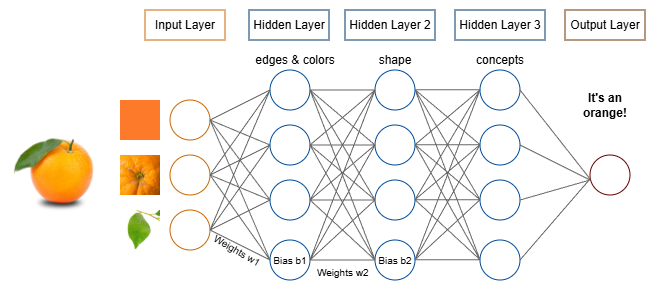
\includegraphics[scale=0.7]{Franzelin_Master/img/ANN_Chart.png}
    \caption{Schematic structure of a fully connected artificial neural network.}
    \label{fig:ann_chart}

\end{figure}

Each neuron calculates a weighted sum of all the incoming inputs and adds a bias. Then a non-linear activation function is applied. In Figure~\ref{fig:ann_chart}, the arrows represent the weights $W^{(l)}_{ji}$, the circles represent the activations $h^{(l)}_{j}$, and the labels bias $b^{(l)}$ indicating the bias associated with each neuron. Input patches from the orange image correspond to $h^{(0)}_{i}$. The forward pass can be written as \citep{Montesinos2022Multivariate}:

\begin{equation}
h^{(l)}_{j} = g^{(l)}\!\left( \sum_{i} W^{(l)}_{ji}\, h^{(l-1)}_{i} + b^{(l)}_{j} \right)
\label{eq:neuron_forward_pass}
\end{equation}



This layered representation learning is the core mechanism that underlies all modern deep learning architectures: from convolutional neural networks (CNNs) to transformer-based models, and further to large visual foundation models and multimodal models used in this work.

\subsection{Convolutional Neural Networks (CNNs)}
\label{sec:cnn_foundations}

As an illustrative example for explaining artificial neural networks (ANNs), the classification of an image of an orange was used. However, this example only serves to introduce the general principles of representation learning; in practice, simple fully connected ANNs are not suited to processing raw image data efficiently \citep{o2015introduction}. Image interpretation requires architectures that explicitly exploit spatial structure, most prominently Convolutional Neural Networks (CNNs) \citep{o2015introduction, Li2021Asurvey}.

CNNs build on the same basic principles as ANNs but introduce architectural constraints that make them capable of handling image-specific tasks \citep{o2015introduction}. The core challenge lies in the high dimensionality of image data \citep{zhang2023dive}. For example, a 1-megapixel image corresponds to 1{,}000{,}000 input features; mapping these to 1{,}000 hidden units in a fully connected layer would require
\[
10^{6} \times 10^{3} = 10^{9},
\]
parameters—computationally infeasible to train \citep{zhang2023dive}.

CNNs overcome this limitation by preserving the spatial structure of an image. Instead of flattening the image into a one-dimensional vector, they represent it as a three-dimensional volume defined by height, width, and depth, where the depth corresponds to the learned feature maps \citep{o2015introduction}.

\begin{figure}[htb]
	\centering  
	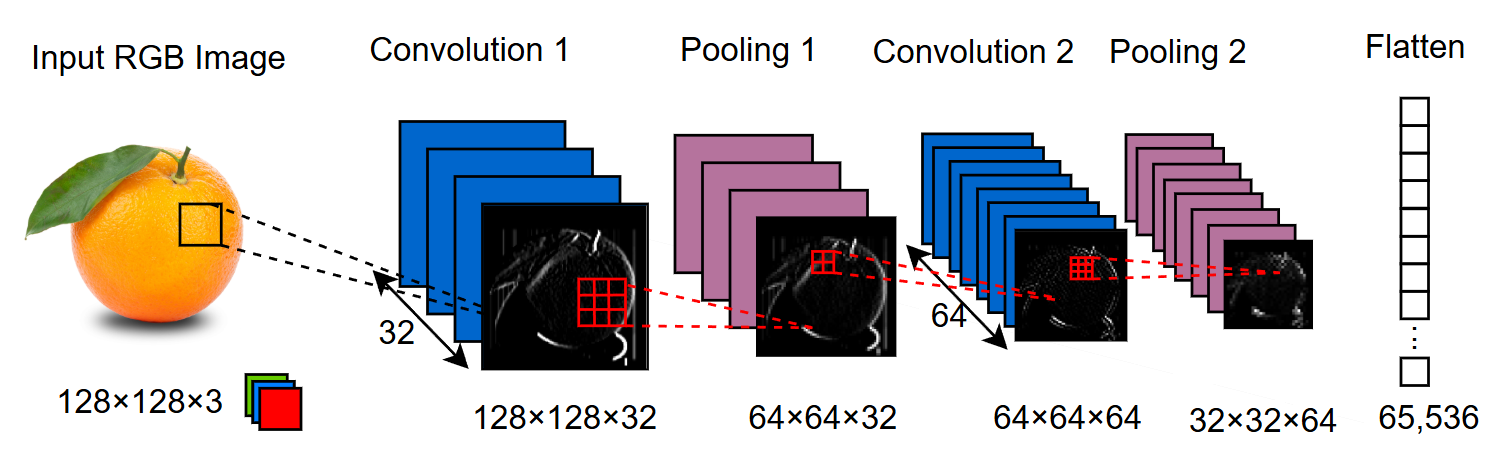
\includegraphics[scale=0.4]{Franzelin_Master/img/CNN_Chart.png}
    \caption{Overview of a Convolutional Neural Network (CNN) architecture.}
    \label{fig:cnn_chart}

\end{figure}

\textbf{Input layer:}

The input layer can be understood as a data container that holds the raw input—in this case, an image of an orange. It stores all pixel values in a tensor with a defined height, width, and number of channels (RGB). In Figure~\ref{fig:cnn_chart}, the input therefore has the shape \(128 \times 128 \times 3\).

\textbf{Convolutional layer:}


Convolutions reduce the complexity and size of the input by optimizing how information is processed and represented \citep{o2015introduction}. A filter (a small square matrix), also called a kernel, slides across the image from top-left to bottom-right and detects local patterns in the pixel values of the input image \citep{Montesinos2022Multivariate}. When the values in the image patch and the kernel align well, the resulting dot product is large; when they differ, the response remains low as shown in Equation~\ref{eq:conv_example}
. The collection of these responses across all positions forms the activation map (also known as the feature map) \citep{Montesinos2022Multivariate}.

\begin{equation}
\text{Response} 
= 
\sum 
\left(
\underbrace{
\begin{bmatrix}
100 & 103 & 100 \\
102 & 105 & 101 \\
98  & 99  & 97
\end{bmatrix}
}_{\text{Patch}}
\;\odot\;
\underbrace{
\begin{bmatrix}
1 & 0 & -1 \\
1 & 0 & -1 \\
1 & 0 & -1
\end{bmatrix}
}_{\text{Kernel}}
\right)
= 2
\label{eq:conv_example}
\end{equation}

\textbf{Pooling layer:}

The purpose of a pooling layer is to downsample the feature maps without introducing additional trainable parameters \citep{Montesinos2022Multivariate, o2015introduction}. Typically, a 2×2 kernel moves across the activation map and selects the largest value within each local patch (max pooling). This reduces the spatial resolution and therefore the computational complexity, while preserving the most important information. By discarding exact spatial locations and retaining only whether a pattern is present, pooling increases robustness to small spatial shifts \citep{Montesinos2022Multivariate}. Stride is the variable determining the stepsize of the kernel moving across the patch/feature map.
\begin{figure}[h]
\centering
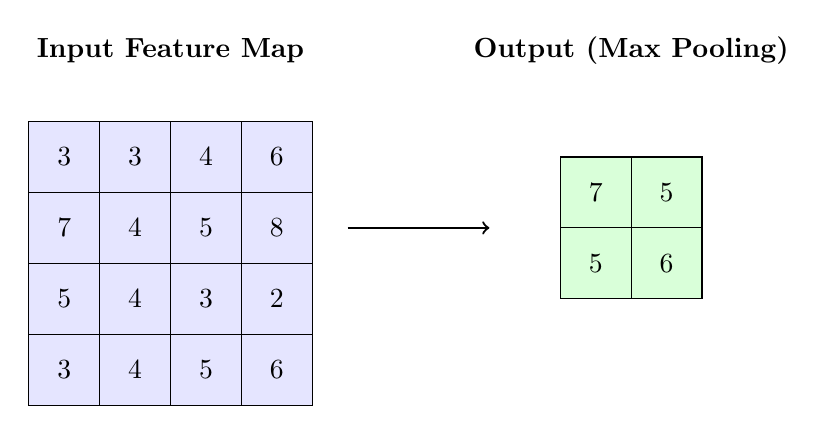
\begin{tikzpicture}[scale=0.9]

% --- Input matrix (4x4) ---
\foreach \i/\row in {1/{3,3,4,6},
                     2/{7,4,5,8},
                     3/{5,4,3,2},
                     4/{3,4,5,6}} {
    \foreach \j [count=\k] in \row {
        \node[draw, minimum size=0.9cm, fill=blue!10] (a\i\k) at (\k, -\i) {\j};
    }
}

\node at (2.5,0.5) {\textbf{Input Feature Map}};

% --- Arrow ---
\draw[->, thick] (5,-2) -- (7,-2);

% --- Output matrix (2x2 max-pooled) ---
\foreach \i/\row in {1/{7,5},
                     2/{5,6}} {
    \foreach \j [count=\k] in \row {
        \node[draw, minimum size=0.9cm, fill=green!15] (b\i\k) at (7.5+\k, -\i-0.5) {\j};
    }
}

\node at (9,0.5) {\textbf{Output (Max Pooling)}};

\end{tikzpicture}
\caption{Example of \(2 \times 2\) max pooling with stride 2.}
\label{fig:maxpool_example}
\end{figure}


\textbf{Fully connected layers:}

After flattening the feature maps (Figure~\ref{fig:cnn_chart}), the network transitions into a standard fully connected artificial neural network, described earlier in Section~\ref{sec:ann_representation_learning}, which computes the final prediction.


\subsection{Transformer Models}
\label{sec:transformer_models}

With the paper by \cite{VaswaniTransformerBase}, the foundation was laid for the transformer architecture in deep learning for natural language processing. Instead of relying on the inherently sequential processing of convolutional neural network models, the Transformer was presented as an architecture that uses self-attention to model dependencies between tokens across the entire input sequence \citep{VaswaniTransformerBase}. Further, \cite{DosovitskiyTransformer} extended this idea to computer vision by introducing the Vision Transformer (ViT), which applies the transformer architecture from \cite{VaswaniTransformerBase} directly to image recognition. In their approach, an image is divided into a sequence of fixed-size patches that are linearly embedded and processed as tokens by a standard transformer encoder \citep{DosovitskiyTransformer}. To understand how such vision transformers operate, the following paragraphs briefly summarise the core building blocks of a transformer encoder:

\textbf{Tokenizer:} The natural language input is first split into tokens \(x_1,\dots,x_n\) (words or, more commonly, subword units), and each token is mapped to a unique integer ID \(\mathrm{id}_i\) from a fixed vocabulary \citep{tunstall2022naturaltransformer, VaswaniTransformerBase}.
Using an embedding lookup table, each ID \(\mathrm{id}_i\) is converted into a dense token embedding vector \(e_i \in \mathbb{R}^{d_{\text{model}}}\), which represents the token content in the model’s feature space. \citep{tunstall2022naturaltransformer}

\begin{figure}[htb]
	\centering
	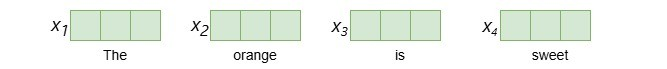
\includegraphics[scale=0.7]{Franzelin_Master/img/Tokinarization.jpg}
	\caption{Illustration of tokenization and mapping tokens to integer IDs (and their token embeddings).}
	\label{fig:tokenization}
\end{figure}

\textbf{Positional embeddings:} Since self-attention alone does not encode the order of tokens, positional information is added to the token embeddings so the model can represent the relative or absolute position of each token in the sequence \citep{tunstall2022naturaltransformer, VaswaniTransformerBase}.
Concretely, each position \(i\) is associated with a positional embedding \(p_i \in \mathbb{R}^{d_{\text{model}}}\).
The final input embedding for the encoder is then obtained by combining token and position information, typically via element-wise addition:
\begin{equation}
x_i^{(0)} = e_i + p_i \,, \qquad i=1,\dots,n \, .
\end{equation}

\begin{figure}[htb]
	\centering
	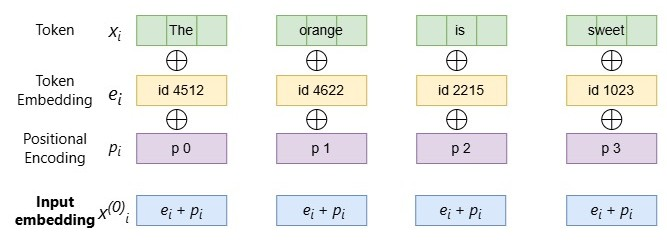
\includegraphics[scale=0.7]{Franzelin_Master/img/InputEmbeding.jpg}
	\caption{Input embedding construction: the token embedding \(e_i\) is combined with the positional embedding \(p_i\) to form the encoder input \(x_i^{(0)}\).}
	\label{fig:input_embedding}
\end{figure}


\textbf{Self-attention:} The self-attention layer assigns a different amount of weight (or attention) to each token embedding by comparing every token to every other token in the same sequence \citep{tunstall2022naturaltransformer}. For each token \(x_i\), self-attention computes weights \(w_{ji}\) that quantify how strongly token \(j\) should contribute to the update of token \(i\), yielding a contextualized representation \citep{tunstall2022naturaltransformer}
\begin{equation}
x_i^{(1)} = \sum_{j=1}^{n} w_{ij}\, x_j^{(0)} \, .
\label{eq:self_attention_weighted_sum}
\end{equation}

A key role in computing the weights is played by the \emph{query}, \emph{key}, and \emph{value} representations.
From an information-retrieval perspective, attention can be seen as a \emph{soft} database lookup: a query is matched against keys, and the output is formed by aggregating the corresponding values \citep{ghojoghAttentionMechanism}.
In this sense, the query \(Q\) encodes what a token is looking for, the key \(K\) describes what a token offers for matching, and the value \(V\) contains the information that is mixed into the resulting representation \citep{tunstall2022naturaltransformer}.

In the scaled dot-product formulation, attention scores are computed by comparing queries and keys (typically via dot products), scaled, and then normalized with a softmax to obtain weights that sum to one \citep{VaswaniTransformerBase}.
\cite{VaswaniTransformerBase} express this in matrix form as
\begin{equation}
\mathrm{Attention}(Q,K,V) \;=\; \mathrm{softmax}\!\left(\frac{QK^{\top}}{\sqrt{d_k}}\right) V \, .
\end{equation}

\begin{figure}[htb]
	\centering  
	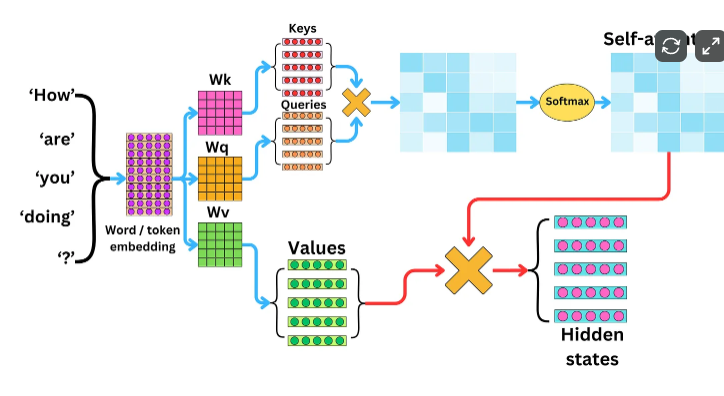
\includegraphics[scale=0.7]{Franzelin_Master/img/SelfAttention.png}
    \caption{Illustration used to explain self-attention between tokens.}
    \label{fig:self_attention}

\end{figure}


For example, consider the token sequence \(x_1=\) ``The'', \(x_2=\) ``orange'', \(x_3=\) ``is'', \(x_4=\) ``sweet'', as illustrated in Figure~\ref{fig:self_attention}. When updating the representation of \(x_2\) (``orange''), the model may assign a relatively large attention weight \(w_{2,4}\) to \(x_4\) (``sweet''), since the adjective conveys an important attribute of the noun, while assigning a smaller weight to \(x_1\) (``The''), which contributes little semantic information about the object. Conversely, when updating \(x_4\) (``sweet''), the model can attend strongly to \(x_2\) (``orange'') (i.e., a high \(w_{4,2}\)) to attach the
property ``sweet'' to the correct entity rather than spreading it across less relevant tokens.




% TODO: Improve or redraw the self-attention illustration if needed.

\textbf{Multi-head attention:} Multi-head attention splits the self-attention mechanism into \(N_h\)
parallel heads, where each head has its own learned projections and computes attention on a lower-dimensional subspace; the resulting head outputs are then concatenated and linearly projected back to the model dimension \citep{VaswaniTransformerBase,tunstall2022naturaltransformer}. Different heads can focus on different relations in the data for example, one head may concentrate on short-range syntactic dependencies, while another captures longer-range semantic links, or in images one head may specialize in edges while another emphasizes textures. Building on this, \cite{CordonnierMultiHeadAtttention} observe that many heads learn redundant query/key projections and propose a \emph{collaborative} multi-head attention variant, in which heads share common projection matrices and differ only by learned mixing vectors; this reduces the number of parameters in the attention layer while maintaining model expressivity.

\textbf{Feed-forward network (FFN):} The feed-forward layer is a two-layer fully connected neural network, similar to the artificial neural network explained in Section~\ref{sec:ann_representation_learning} \citep{VaswaniTransformerBase}. It takes the contextualized token embeddings from self-attention as input and applies the same small MLP independently to each token position: first expanding to a larger hidden dimension (typically 4× the embedding size), then applying a non-linear activation (GELU), and finally projecting back to the original embedding size \citep{tunstall2022naturaltransformer}.

\textbf{Residual connections and layer normalization:}  
Residual connections and layer normalization are key components in transformer architectures that stabilize training and improve information flow \citep{VaswaniTransformerBase, ba2016layernormalization, he2015deepresiduallearningimage}.

Residual connections introduce shortcut paths by adding the input of a sublayer to its output, i.e.,
\[
x + \mathrm{Sublayer}(x) \, .
\]
Originally introduced in deep residual networks \citep{he2015deepresiduallearningimage}, this mechanism facilitates gradient propagation, mitigates the vanishing gradient problem, and helps preserve information across layers. In transformers, residual connections are applied around each sublayer \citep{VaswaniTransformerBase}.

Layer normalization stabilizes activations by normalizing them to zero mean and unit variance, followed by a learnable scaling and shifting \citep{ba2016layernormalization}. This reduces numerical instability and accelerates convergence, particularly in sequence models such as transformers \citep{VaswaniTransformerBase}.

Two common arrangements exist. In the original \emph{Post-LN} formulation used in the transformer, normalization is applied after the residual addition:
\[
\mathrm{LayerNorm}(x + \mathrm{Sublayer}(x)) \, .
\]
Modern architectures often use \emph{Pre-LN}, where normalization is applied before the sublayer:
\[
x + \mathrm{Sublayer}(\mathrm{LayerNorm}(x)) \, ,
\]
which generally improves training stability and simplifies optimization in deep transformer models \citep{ba2016layernormalization}.

\subsection{Transformer Architectures in Computer Vision}

Although the transformer architecture was originally introduced for natural language processing by \cite{VaswaniTransformerBase}, its ability to model global dependencies through self-attention makes it highly suitable for computer vision tasks as well. Unlike convolutional neural networks (CNNs), which rely on local receptive fields and hierarchical feature extraction, transformers can directly capture long-range relationships across the entire input \citep{pereira2024reviewtransformerbasedmodelscomputer}. In this work, particular focus is placed on the \emph{Vision Transformer (ViT)} \citep{DosovitskiyTransformer}, as it forms the architectural foundation of many modern vision models, including both the multimodal model (Qwen-VL) and the segmentation model (SAM) used in this thesis.

\textbf{Vision Transformer (ViT):}
A Vision Transformer divides an image into fixed-size patches, linearly embeds each patch, and processes the resulting sequence of visual tokens with a transformer encoder \citep{DosovitskiyTransformer}. This allows self-attention to be applied to image data and makes it possible to model relationships between distant image regions. ViT-like encoders are relevant for this thesis because they form the visual backbone of many multimodal and segmentation foundation models.


\section{Foundation Models}
\label{sec:foundation_models}

First, it is necessary to define what a foundation model is in the context of deep learning. Although foundation models rely on the same fundamental architectures introduced in Section~\ref{sec:deep_learning_foundations}, such as CNNs and transformer-based models, they differ primarily in their scale of training. A foundation model refers to a model that is trained on very large amounts of general-purpose data and can subsequently be adapted to a wide range of downstream applications through fine-tuning or prompting \citep{bommasani2022opportunitiesrisksfoundationmodels, Schneider2024}. As models are trained with billions of parameters and extremely large training datasets, they increasingly demonstrate the ability to perform tasks for which they were not explicitly trained \citep{Brown2020FoundationModelFewShot, bommasani2022opportunitiesrisksfoundationmodels}.
Large-scale foundation models often exhibit unexpected capabilities, such as reasoning, translation, mathematical problem solving, or analogical reasoning, even though these abilities were not explicitly targeted during training \citep{Brown2020FoundationModelFewShot}. Different usage settings can be distinguished depending on how much task-specific information is provided. In the case of fine-tuning, the model weights are updated using a task-specific dataset, which typically requires thousands of labeled examples. In contrast, zero-shot learning performs a task without any examples, relying only on an instruction. One-shot learning provides a single example, while few-shot learning supplies a small number of examples (usually between 10 and 100) within the prompt \citep{Brown2020FoundationModelFewShot}.

\cite{bommasani2022opportunitiesrisksfoundationmodels} describe two central characteristics of foundation models: emergence and homogenization. Emergence refers to capabilities that appear only at larger model scales, while homogenization describes the increasing reliance of many AI systems on a small number of shared base models. This can improve efficiency and transferability, but it also creates the risk that errors, biases, or limitations of the base model propagate into many downstream applications.

 Examples of such foundation models include systems such as ChatGPT, Claude, Qwen-VL, and LLaMA. Many of these systems are multimodal large language models that are trained primarily on text but can also process images and other data modalities. In addition to multimodal language models, there also exist visual foundation models that are designed specifically for image understanding tasks. One example is the Segment Anything Model (SAM) developed by Meta, which was trained on billions of images and segmentation masks to enable general-purpose image segmentation \citep{kirillov2023segment}.

From a technological standpoint, foundation models do not fundamentally differ from traditional deep learning approaches in terms of their core architectures. Both rely on neural network architectures such as convolutional neural networks and transformer-based models. The main difference lies in the training paradigm and the deployment workflow \citep{bommasani2022opportunitiesrisksfoundationmodels, Schneider2024}.
\begin{figure}[htb]
	\centering  
	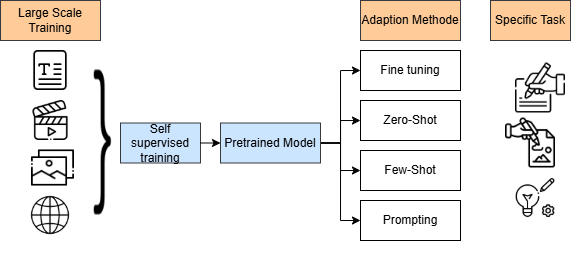
\includegraphics[scale=0.6]{Franzelin_Master/img/foundationmodel.drawio.png}
	\caption{Illustration used to explain the concept of foundation models and downstream adaptation.}
	\label{fig:foundation_model_overview}
\end{figure}
Foundation models are typically trained using self-supervised learning on very large and diverse datasets. This training strategy allows the model to learn general representations of the data without requiring manually labeled annotations. Instead, the model is trained using proxy tasks, such as predicting the next token in a sequence for language models or reconstructing masked regions in images for vision models. Through these objectives, the model gradually learns semantic structures and patterns present in the training data \citep{bommasani2022opportunitiesrisksfoundationmodels}.

After this large-scale pretraining phase, the resulting model can be adapted to specific downstream tasks through different mechanisms \citep{bommasani2022opportunitiesrisksfoundationmodels}. These include fine-tuning, where the model weights are updated using labeled task-specific data, as well as prompting techniques, where task instructions are provided as input without modifying the model parameters \citep{Brown2020FoundationModelFewShot}.

The concept of foundation models can also be illustrated using the earlier fruit example. In a traditional supervised learning setting, a neural network might be trained specifically to distinguish between apples and oranges using a labeled dataset. The model therefore learns a very narrow task: binary fruit classification. In contrast, a foundation model is trained on a much larger and more diverse dataset containing many different types of objects, scenes, and contexts. Instead of learning only the distinction between apples and oranges, the model learns general visual concepts such as color patterns, textures, shapes, and object boundaries across thousands or millions of object categories.

\subsection{Multimodal Large Language Models (MLLMs)}
\label{sec:mllm_foundations}

Multimodal Large Language Models (MLLMs) are language models that are capable of processing and understanding information from multiple modalities, such as text, images, audio, or video. They can be understood as a combination of Large Language Models (LLMs) and Large Vision Models (LVMs). LLMs focus on natural language processing tasks and exhibit capabilities such as instruction following, in-context learning, and advanced reasoning abilities \citep{Brown2020FoundationModelFewShot}. In contrast, LVMs primarily focus on visual perception tasks, including object recognition and image understanding \citep{Yin_2024MLLM}.

The development of modern LLMs was enabled by the introduction of the transformer architecture \citep{VaswaniTransformerBase}, which allows models to efficiently process long sequences and capture complex dependencies in textual data. In addition, advances in large-scale self-supervised learning have significantly contributed to the success of these models, allowing them to learn general representations from massive unlabeled datasets \citep{xiao2025foundationslargelanguagemodels}.

\begin{figure}[htb]
	\centering  
	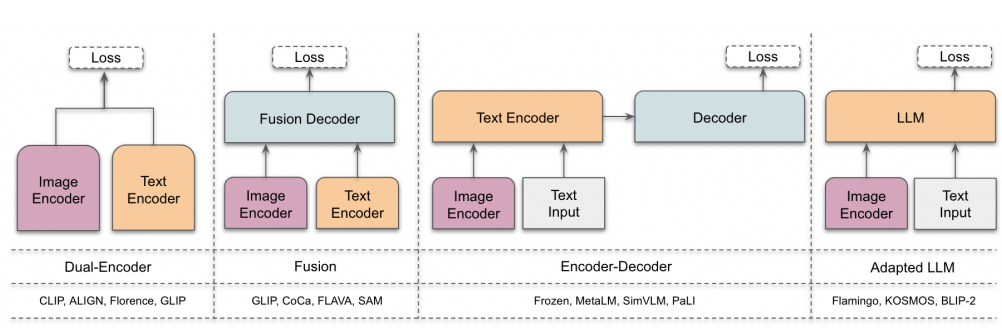
\includegraphics[scale=0.8]{Franzelin_Master/img/mllm_differentarchitectures.png}
	\caption{General architecture of a multimodal large language model integrating textual and multimodal inputs through modality-specific encoders and a language model backbone.}
	\label{fig:mllm_architecture_overview}
\end{figure}

Architecturally, most Multimodal Large Language Models (MLLMs) extend pretrained transformer-based language models \citep{liang2025comprehensivesurveyguidemultimodal}, as introduced in Section~\ref{sec:transformer_models}.
Text inputs are processed through the standard language modeling pipeline consisting of tokenization and embedding, while non-textual inputs such as images or videos are processed by modality-specific encoders that transform raw sensory inputs into dense feature representations \citep{Yin_2024MLLM}.

Different architectural paradigms have been proposed for vision-language models. 
According to \cite{awais2023foundationalmodelsdefiningnew}, four main architecture types can be distinguished: dual-encoder, fusion-based, encoder–decoder, and adapter-based LLM architectures. 
The dual-encoder architecture processes visual and textual inputs with separate encoders and aligns their representations within a shared embedding space. 
Fusion architectures introduce an additional module that jointly combines image and text features to learn richer cross-modal representations. 
Encoder–decoder architectures first extract visual features using a vision encoder and subsequently generate textual outputs through a decoder-based language model. 
Finally, adapter-based LLM architectures employ a large language model as the central component and use modality-specific encoders to convert visual inputs into representations that can be processed together with textual tokens by the LLM \citep{awais2023foundationalmodelsdefiningnew}.

Among the different architectural paradigms, adapter-based LLM architectures have recently become the dominant approach for multimodal large language models. 
This design is employed by several widely used models such as LLaVA and GPT-4V, and is also adopted by the model used in this work, Qwen3-VL-8B-Instruct.

\begin{figure}[htb]
	\centering  
	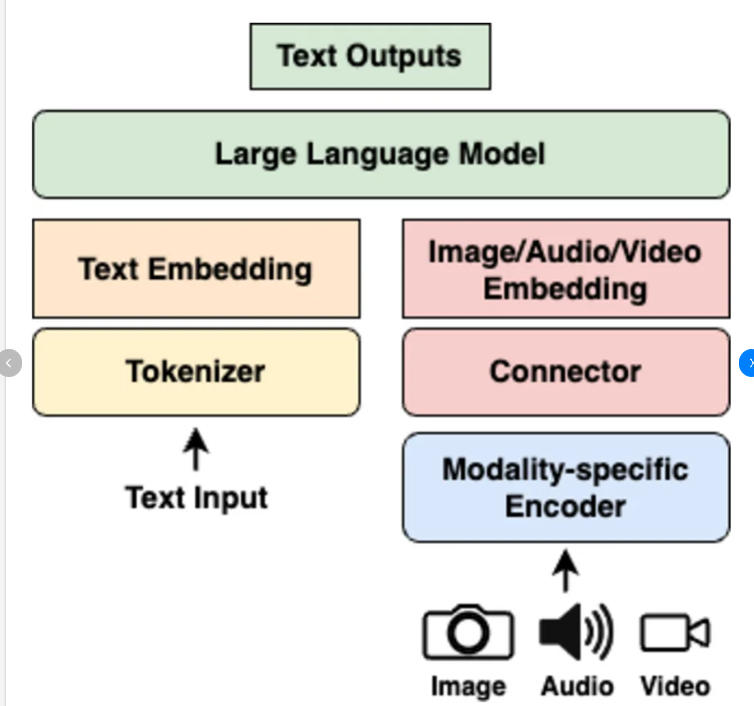
\includegraphics[scale=0.8]{Franzelin_Master/img/mllmarchitecture.png}
	\caption{General architecture of a multimodal large language model integrating textual and multimodal inputs through modality-specific encoders and a language model backbone.}
	\label{fig:mllm_adapter_architecture}
\end{figure}


First, a \textbf{modality-specific encoder} converts raw inputs, such as images, into feature embeddings that can be processed by the model. 
Typical implementations include vision encoders such as Vision Transformers (ViT) or convolutional neural network (CNN) backbones \citep{liang2025comprehensivesurveyguidemultimodal}.

Second, a \textbf{projection or alignment module} transforms the encoded visual features into a representation that is compatible with the embedding space of the language model. 
This step aligns the visual features with textual tokens, allowing the model to process both modalities jointly. 
Common approaches include projection layers or resampling modules that convert visual embeddings into token-like representations \citep{liang2025comprehensivesurveyguidemultimodal}.

Finally, the \textbf{language model backbone} processes the combined sequence of textual and visual tokens.  Using the transformer architecture \citep{VaswaniTransformerBase}, the language model integrates the multimodal information and performs reasoning or generation tasks \citep{liang2025comprehensivesurveyguidemultimodal}.

\subsubsection{Qwen-VL Multimodal Model}

In this work, the selected vision–language model must be capable of handling several tasks that are essential for building footprint analysis from aerial imagery. In particular, the model needs to perform well in three main capabilities: 

geospatial reasoning, 
spatial error analysis,
and coordinate or point detection.

Geospatial reasoning is required for understanding the spatial structure of buildings and verifying whether predicted polygons follow the outlines of houses correctly. Spatial reasoning is also necessary to analyze potential errors in building footprints, for example identifying cases where a polygon under- or over-segments a roof area. Finally, the model must be able to perform coordinate reasoning in order to place points either on or outside the building structure, which is required for the iterative correction pipeline developed in this thesis.

The selection of the model was primarily based on recent benchmark studies evaluating vision–language models for remote sensing tasks. In particular, the CHOICE benchmark \citep{an2025choicebenchmarkingremotesensing} evaluates several multimodal models on tasks relevant to geospatial reasoning and spatial understanding in remote sensing imagery. As shown in Table~\ref{tab:choice_results}, Qwen2-VL-72B performs strongly across several key capabilities that are relevant to the tasks in this thesis. For example, the model ranks first in spatial relationship reasoning and achieves top-three performance in object localization and visual grounding tasks. These capabilities are directly related to reasoning about building footprints, spatial relationships between objects, and coordinate-level predictions.

\begin{table}[h]
\centering
\caption{Performance of Vision-Language Models on selected tasks from the CHOICE \citep{an2025choicebenchmarkingremotesensing} and GEOBench-VLM \citep{danish2025geobenchvlmbenchmarkingvisionlanguagemodels} benchmarks relevant for geospatial reasoning and building footprint analysis.}
\label{tab:choice_results}
\begin{tabular}{p{3cm} p{4cm} p{5cm} c c}
\hline
\textbf{Benchmark} & \textbf{Capability Dimension} & \textbf{Task Description} & \textbf{Model (Score)} \\
\hline

\multirow{3}{3cm}{CHOICE} 
& \multirow{3}{4cm}{Geospatial Determination (GD)}
& \multirow{3}{5cm}{Inferring geographic context from remote sensing imagery}
 & GLM-4V-9B (0.990) \\
& &  & Gemini-1.5-Pro (0.985) \\
& &  & Qwen2-VL-72B (0.980) \\

\hline

\multirow{3}{3cm}{CHOICE}
& \multirow{3}{4cm}{Spatial Relationship (SR)}
& \multirow{3}{5cm}{Reasoning about spatial relations between objects}
 & Qwen2-VL-72B (0.610) \\
& &  & GPT-4o-2024-11-20 (0.567) \\
& &  & InternVL2-40B (0.500) \\

\hline

\multirow{3}{3cm}{CHOICE}
& \multirow{3}{4cm}{Object Localization (OL)}
& \multirow{3}{5cm}{Identifying object positions in an image}
 & VHM (0.872) \\
& &  & Qwen2-VL-72B (0.840) \\
& &  & InternVL2-40B (0.770) \\

\hline

\multirow{3}{3cm}{GEOBench-VLM}
& \multirow{3}{4cm}{Scene Understanding}
& \multirow{3}{5cm}{Identifying scene types in aerial imagery}
 & EarthDial (0.7705) \\
& &  & GPT-4o (0.7114) \\
& & & Qwen2-VL (0.6761) \\

\hline

\multirow{3}{3cm}{GEOBench-VLM}
& \multirow{3}{4cm}{Object Classification}
& \multirow{3}{5cm}{Recognizing object categories in remote sensing images}
 & GPT-4o (0.5863) \\
& & & LLaVA-OneVision (0.4593) \\
& & & Qwen2-VL (0.4560) \\

\hline

\multirow{3}{3cm}{GEOBench-VLM}
& \multirow{3}{4cm}{Object Localization \& Counting}
& \multirow{3}{5cm}{Detecting and counting objects in aerial imagery}
 & LLaVA-OneVision (0.4377) \\
& &  & Qwen2-VL (0.4019) \\
& &  & GPT-4o (0.3965) \\

\hline
\end{tabular}
\end{table}

In addition to the CHOICE benchmark, the GEOBench-VLM benchmark \citep{danish2025geobenchvlmbenchmarkingvisionlanguagemodels} evaluates vision–language models across a range of geospatial tasks including scene understanding, object classification, and object localization. The results summarized in Table~\ref{tab:choice_results} show that general-purpose multimodal models achieve competitive performance across many geospatial reasoning tasks. Although Qwen2-VL does not always rank first, it consistently performs among the top models across several categories.

Another important consideration in model selection was the difference between domain-specific remote sensing models and general-purpose vision–language models. According to \cite{an2025choicebenchmarkingremotesensing}, many models specifically trained for remote sensing tasks often underperform compared to large general-purpose multimodal models when evaluated on complex reasoning tasks. These models benefit from large-scale multimodal training data and therefore often exhibit stronger visual reasoning and spatial understanding capabilities. Furthermore, practical constraints influenced the model choice. Closed-source models such as GPT-4o and Gemini were excluded because they require paid API access and provide limited transparency regarding model architecture and training data. In contrast, open-source models allow reproducibility, full control over the inference pipeline, and easier integration into custom workflows. Among the remaining candidates, InternVL and Qwen-VL were evaluated within the experimental pipeline developed for this thesis. Empirical testing showed that Qwen-VL produced slightly better results in tasks related to spatial reasoning and object localization. Therefore, Qwen2-VL was selected as the primary multimodal model family during development. During the development of this work, a newer version of the Qwen-VL model family became available. Consequently, the final implementation uses Qwen3-VL-8B-Instruct. Due to computational constraints and hardware availability, the 8B parameter variant was selected. Larger models require significantly more GPU memory and computational resources, which makes them difficult to deploy within a practical and cost-effective research setup.

The architecture and model family of Qwen3-VL are described in the Qwen3-VL technical report \citep{bai2025qwen3vltechnicalreport}. In this thesis, Qwen3-VL-8B-Instruct was selected because it provided a practical compromise between multimodal capability and available computational resources.

% TODO: Add one short paragraph summarizing the relevant Qwen3-VL architecture based on the technical report.
 
\subsection{Visual Foundation Models and Usability for Geospatial Interpretation}

Visual foundation models are trained on large and diverse image datasets and can be adapted to many downstream vision tasks. In geospatial applications, they are relevant because they may reduce the need for task-specific training data and can support segmentation, object localization, and prompt-based image interpretation.

% TODO: Add short paragraph on limitations of visual foundation models in aerial or satellite imagery, including resolution, occlusion, domain shift, and viewing geometry.


\subsubsection{Segment Anything Model (SAM)}

The Segment Anything Model (SAM) is a promptable visual segmentation foundation model introduced by Meta AI \citep{kirillov2023segment}. SAM was trained on the large-scale SA-1B dataset, which contains more than one billion masks, and is designed to produce segmentation masks from prompts such as points, boxes, or masks.

For building-footprint refinement, SAM is relevant because it can generate local segmentation masks for individual buildings based on prompts derived from existing polygons or MLLM-generated points. However, SAM produces raster-like masks rather than clean vector geometries. Building-footprint applications therefore require an additional polygonization and regularization step before the output can be used as GIS-ready vector data.

% TODO: Add one short sentence about SAM3/text-prompted segmentation if this is discussed in the Methods chapter.







\section{Building Footprints}
\label{sec:building_footprints}

Building on the previous discussion of geospatial data quality and automated quality assurance, this thesis now focuses on a specific and widely used geospatial object: building footprints. 

\subsection{Definition and GIS Representation}

Building footprints represent the outline of buildings as vector polygons and form a fundamental component of many spatial datasets. Accurate and up-to-date footprints are required for a broad range of applications, including mapping, urban and regional planning, infrastructure monitoring, population estimation, land-use analysis, and disaster response \citep{Awrangjeb_AutomaticExtraction, sirko2021continentalscalebuildingdetectionhigh}.

\begin{figure}[htb]
	\centering  
	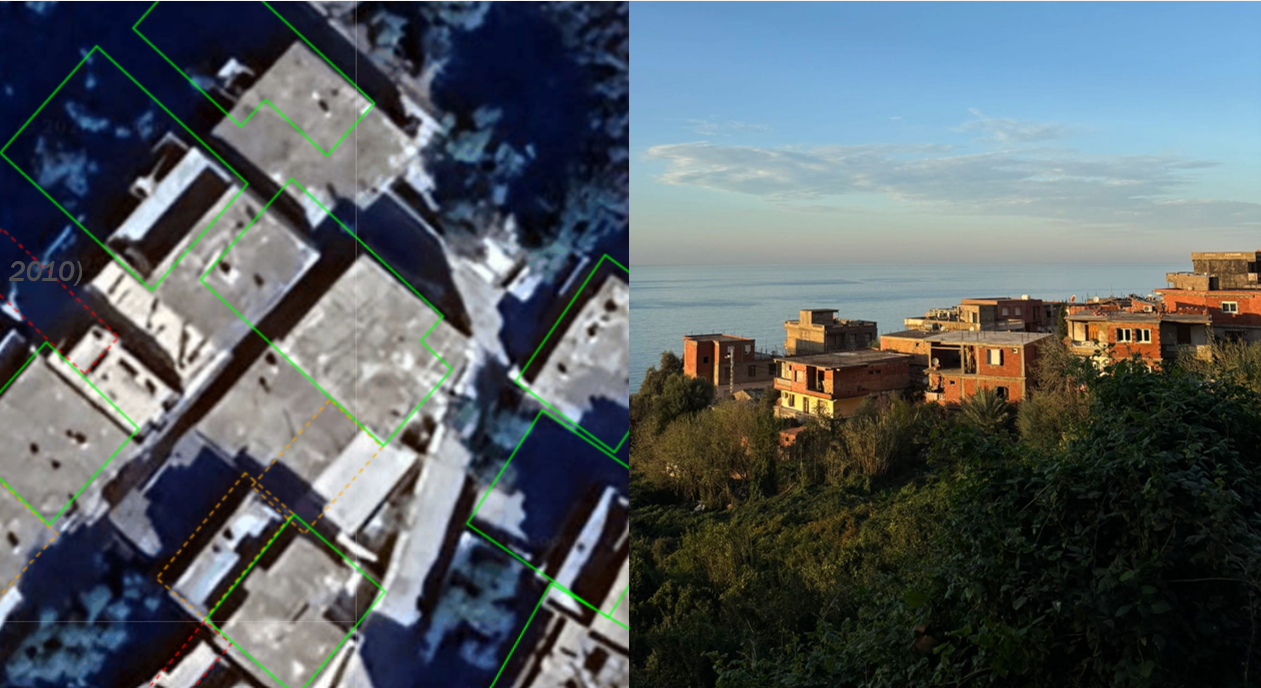
\includegraphics[scale=0.7]{Franzelin_Master/img/Building_Footprint.png}
    \caption{Illustration used to support the discussion of building footprints.}
    \label{fig:building_footprint}

\end{figure}

The technical report accompanying the Google Open Buildings dataset \citep{sirko2021continentalscalebuildingdetectionhigh}, which serves as a baseline for this work, emphasizes the importance of large-scale building footprint data in closing existing information gaps, particularly in developing regions. In such contexts, building footprints are especially valuable in areas with limited or infrequent census coverage, a high prevalence of informal settlements, and rapid urban transformation, as commonly observed in emerging megacities.

In Africa, for example, authoritative national building datasets are largely unavailable, making automated products often the only accessible source of building footprint information \citep{CHAMBERLAIN2024102104}. Currently, four major global building footprint datasets exist: Google Open Buildings, Microsoft Buildings, Ecopia, and OpenStreetMap (OSM). However, these datasets differ substantially in terms of building counts, total building area, and spatial coverage, indicating that available building footprint products are not interchangeable and exhibit strong spatial heterogeneity in completeness and quality \citep{CHAMBERLAIN2024102104}. Google, Microsoft, and Ecopia datasets are generated automatically using convolutional neural networks applied to high-resolution satellite imagery.

OpenStreetMap differs fundamentally from these products as it is based on volunteered geographic information (VGI) and thus relies on human contributors \citep{CHAMBERLAIN2024102104}. However, mapping activity is unevenly distributed across the globe, resulting in pronounced spatial biases and a strong urban focus \citep{herfort2023spatio}. Herfort et al.\ \cite{herfort2023spatio} report substantial regional differences in urban OSM building completeness, with average values of 71\% in Europe and Central Asia, 64\% in North America, but only 30\% in Sub-Saharan Africa, 20\% in Latin America and the Caribbean, 20\% in East Asia and the Pacific, 12\% in the Middle East and North Africa, and 9\% in South Asia.


\subsection{Typical Errors and Quality Challenges in Building Footprint Datasets}
\label{sec:building_errors}

\cite{Hongchao_QualityAssesmentOSM} identify four core quality criteria for assessing building footprint datasets, each of which corresponds to characteristic error patterns observed in practice. Completeness describes the proportion of real-world buildings represented in the dataset and is primarily affected by omission errors, where buildings are missing entirely. Semantic accuracy refers to the correctness of building-related attributes and tags (e.g., building=yes) and captures semantic inaccuracies in classification or attribute assignment. Positional accuracy measures the spatial offset between building footprints and their counterparts in a reference dataset and thus reflects positional displacements, where polygons are systematically or locally shifted relative to reference maps or imagery. Finally, shape accuracy assesses the geometric similarity between building polygons and reference footprints and is commonly impacted by shape simplification or distortion.

In building-footprint datasets, these quality dimensions are closely linked. A missing building is a completeness error, a shifted polygon is a positional accuracy error, and an oversimplified or distorted outline is a shape-accuracy error. In practice, these categories can overlap. For example, a strongly shifted polygon may also appear to have missing or extra parts when compared with the visible roof outline. This makes building-footprint quality assessment more complex than a single accuracy score and motivates the multi-label error taxonomy used in this thesis.

\textbf{Errors in the Google Open Buildings dataset.}

In the technical report accompanying the Google Open Buildings dataset, Google Research explicitly documents several recurring error types observed during continental-scale building extraction from high-resolution satellite imagery \citep{sirko2021continentalscalebuildingdetectionhigh}. These include difficulties with large buildings, which are sometimes split into multiple instances; complex roof structures, where intricate geometry leads to fragmented or incomplete footprints; and touching or densely packed buildings, for which true boundaries are ambiguous even to human annotators. Additional challenges arise from ambiguous segmentation in visually noisy contexts, tree occlusion that partially conceals rooftops, and confusing natural features (e.g. rocks or bare soil) that can be falsely detected as buildings. Finally, the vectorization process may introduce shape distortions, such as round buildings being approximated as rectangular polygons.

\begin{figure}[htb]
	\centering  
	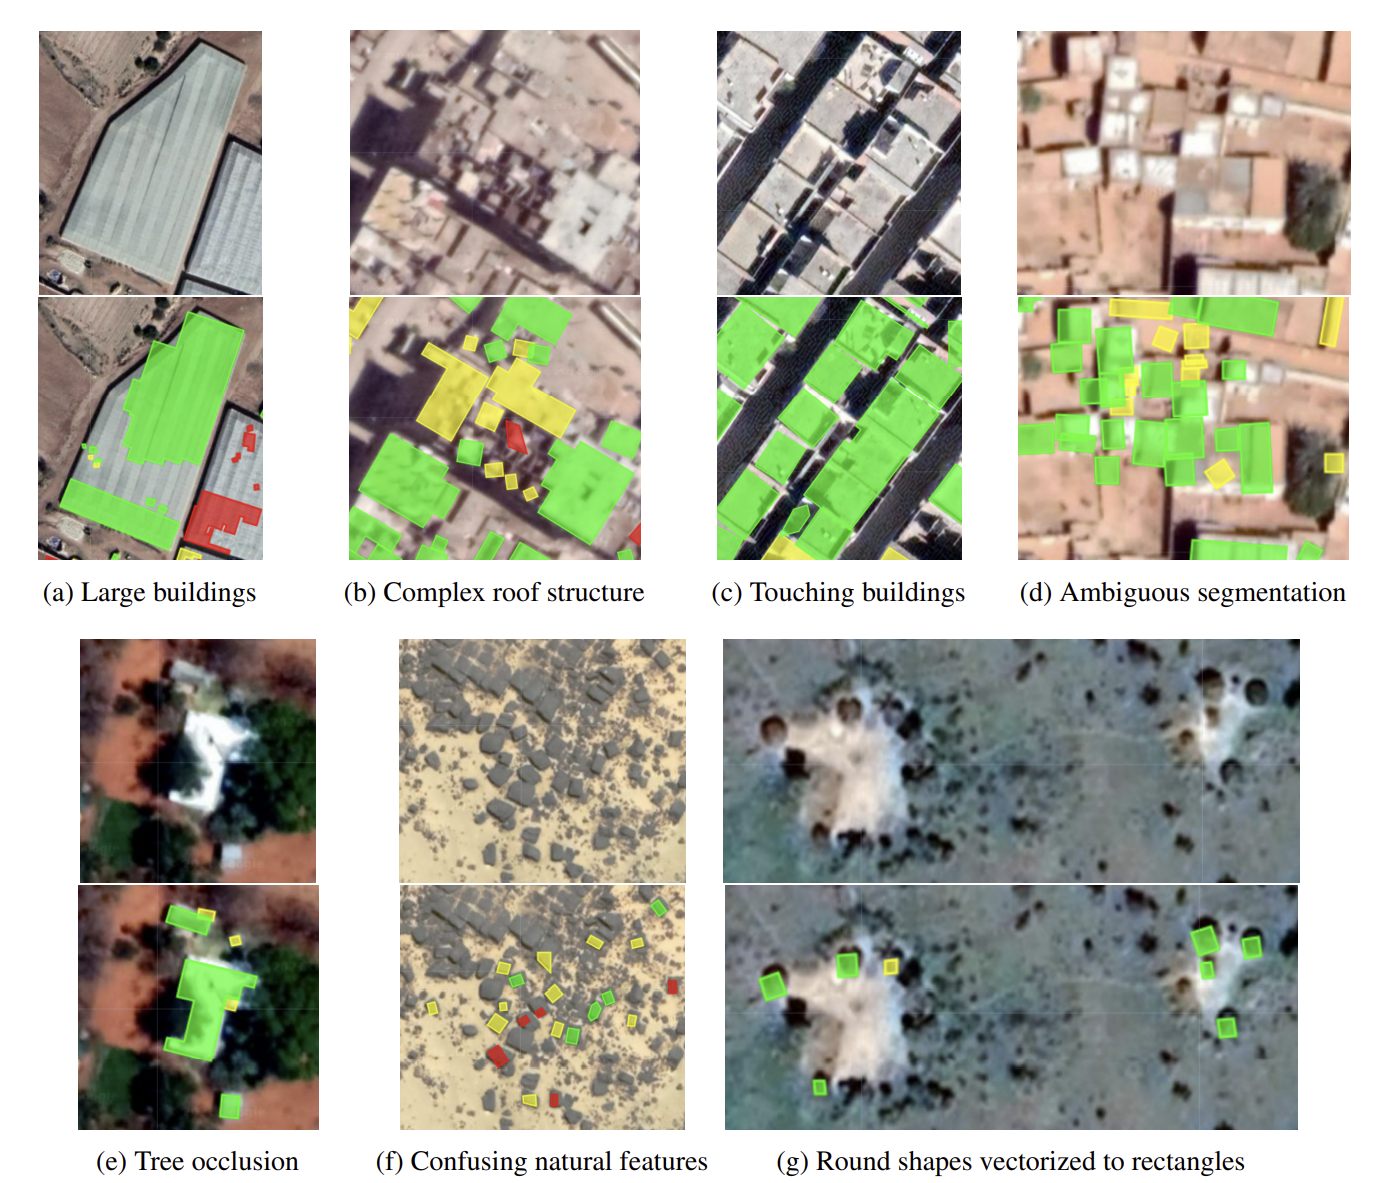
\includegraphics[scale=0.7]{Franzelin_Master/img/googleopenbuildingerrors.png}
    \caption{Illustration used to support the discussion of typical Google Open Buildings errors.}
    \label{fig:google_open_buildings_errors}

\end{figure}

\subsection{Existing QA Approaches}

As discussed in Section~\ref{sec:geospatial_data_quality}, the quality of geospatial features—particularly building footprints—directly affects downstream analysis and decision-making. Traditional QA relies on manual inspection by comparison with original maps or imagery, the use of metadata to document data lineage and uncertainty over time, and geographical consistency checks based on spatial logic (e.g., rivers should not cross contour lines)~\citep{chen2022reviewing}. Based on previous reviews \citep{chen2022reviewing, prodobnukar_actualandprecivedqulity}, existing QA approaches can be broadly grouped into (i) rule-based geometric and topological validation, (ii) sampling and visual inspection against reference data, (iii) metadata-driven quality documentation, and (iv) increasingly automated frameworks that combine multiple evaluation techniques.

A representative example of classical deterministic QA is provided by \cite{ahmed2023qualitymanagement}, who presents specification-driven quality control workflows for GIS databases based on predefined acceptance criteria, geometric and topological consistency rules, attribute validation, edge matching, and structured QA/QC checklists. His framework combines automated validation (e.g., schema conformity, positional accuracy, and attribute completeness) with manual visual inspection and random sampling, reflecting a rule-based approach in which data quality is assessed against explicit standards and thresholds.

More recently, research has begun to explore data-driven alternatives to traditional deterministic quality assurance methods, where machine learning and AI are employed to identify errors and inconsistencies in large datasets. Pysmennyi et al.~\cite{Pysmennyi_2025AI_quality} investigate AI-driven quality assurance in software systems and show that rule-based inspections with fixed acceptance criteria break down under increasing system complexity, rapid development cycles, and growing data volumes. Similarly, in the context of visual quality assurance, Hoffmann and Reich~\cite{Hoffmann_VisualQualityAssurance} show that contemporary visual quality assurance is dominated by deep-learning approaches, particularly CNN-based classification, segmentation, and anomaly detection, largely replacing traditional manual inspection and rule-based computer vision pipelines.

<<<<<<< HEAD
Building-footprint quality assessment often focuses on comparing the dataset under evaluation with a reference dataset. For example, \cite{Hongchao_QualityAssesmentOSM} evaluated the OSM building footprint dataset for Munich by comparison with ATKIS, the authoritative German topographic database. Similarly, \cite{Brovelli_OSM_SpatialAccuracy} validated OSM building footprints for the Lombardy region in northern Italy against an authoritative reference dataset, the Lombardy Regional Topographical Database. However, this reference-based evaluation paradigm raises a fundamental question: how can building footprint quality be assessed in regions where no high-quality authoritative reference dataset is available? One recent study that attempts this for automatically derived global datasets is presented by \cite{okyere2025evaluating}, who compare Google Open Buildings and Microsoft building footprints against OSM across five cities — Accra, Nairobi, Caracas, Berlin, and Houston using metrics such as overlap analysis, relative positional accuracy, and Intersection over Union to identify differences in completeness and spatial alignment without relying on an authoritative cadastral reference layer.

% TODO: Add one short paragraph on rule-based building-footprint QA checks such as minimum area, overlap, duplicate geometries, invalid topology, compactness, and rectangularity.
